\section{Introduction}

GLIMMER\footnote{GENIE Land-Ice Model with Multiply Enabled Regions} is the land ice component of GENIE\footnote{Grid-ENabled Integrated Earth-system model}. Its design is motivated by the desire to create an ice modelling system which is easy to interface to a wide variety of climate models, without the user having to have a detailed knowledge of its inner workings. This is accomplished by providing a very well-defined interface, which allows access to all the functionality required by the user. All model fields and time-dependent parameters required by the ice model are passed to it through the argument lists of the supplied subroutines. Initialisation data is supplied through namelist files, while netCDF files are used for platform independent binary I/O. 

\subsection{Overview}
GLIMMER consits of two components:
\begin{enumerate}
 \item {\bf GLIDE:} This component is the actual ice sheet model. GLIDE is responsible for calculating ice velocities, internal ice temperature distribution, isostatic adjustment and melt water production.
 \item {\bf Climate Drivers:} GLIDE is coupled to the outside world via two fields describing the ice surface temperatures and mass balance and (optionally) a scalar value for eustatic sea level. These drivers can be derived from simple assumptions, e.g. uniform mass balance or EISMINT tests, or from climate model output, e.g. GENIE or a regional climate model.
\end{enumerate}
These components and how their relations are outlined in Figure \ref{ug.glide}.

\begin{figure}[htb]
 \begin{center}
   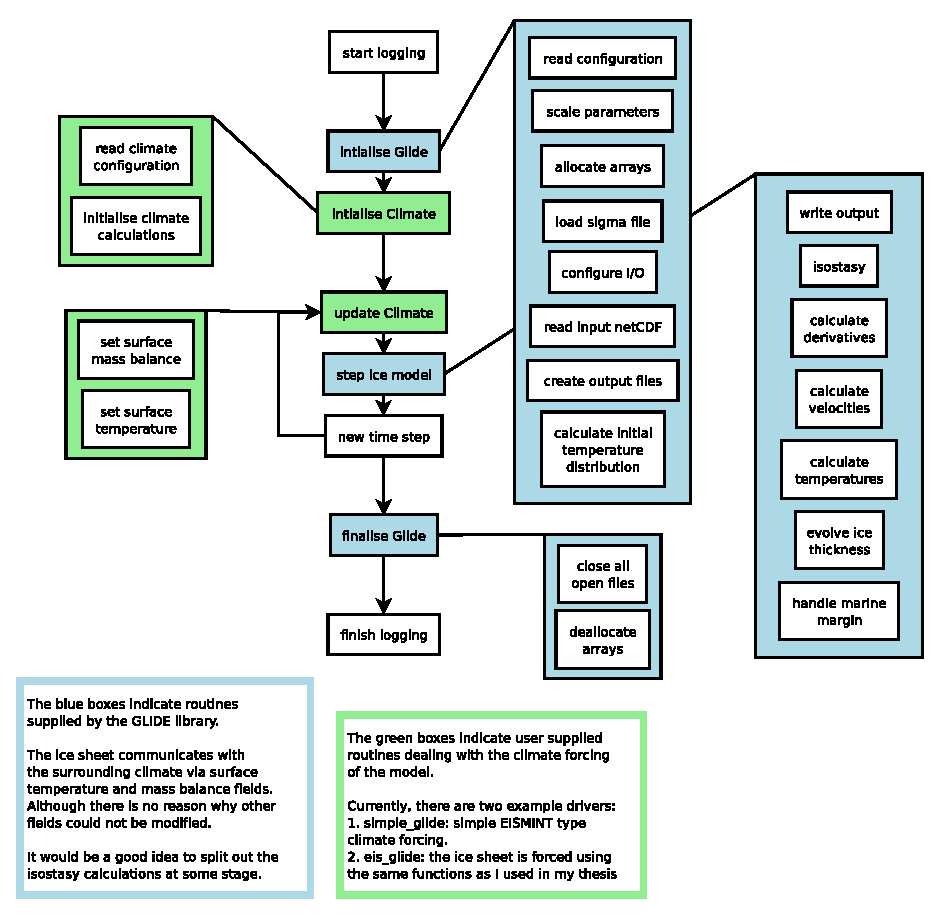
\epsfig{file=\dir/figs/glide.eps,width=0.9\textwidth}
 \end{center}
 \caption{Outline of the GLIDE and Climate components.}
\label{ug.glide}
\end{figure}

Three climate drivers are provided by the GLIMMER module:
\begin{enumerate}
 \item \texttt{simple\_glide}: an EISMINT type driver
 \item \texttt{eis\_glide}: Edinburh Ice Sheet driver. 
 \item \texttt{libglint}: interface to GENIE
\end{enumerate}

\subsection{Configuration, I/O and Visualisation}
Each component is configured using a configuration file similar to Windows \texttt{.ini} files. The model configuration is printed to a log file. 

2D and 3D data is read/written to netCDF files using the CF convention. netCDF is scientific data format for storing multidimensional data in a platform and language independent binary data format. The CF conventions specify the meta data used to describe the file contents.

Many programs can process and visualise netCDF data, e.g. OpenDX. Additionally, the GLIMMER module contains GMT scripts written in Python to visualise the output.

\subsection{Can I use GLIMMER with my climate model?}
We hope so! The external interface of GLIMMER is designed to be quite
flexible, but certain assumptions have necessarily been made about the form
taken by input fields, etc. Check out the climate drivers for examples of varying complexity.

